% Options for packages loaded elsewhere
% Options for packages loaded elsewhere
\PassOptionsToPackage{unicode}{hyperref}
\PassOptionsToPackage{hyphens}{url}
\PassOptionsToPackage{dvipsnames,svgnames,x11names}{xcolor}
%
\documentclass[
  authoryear,
  preprint]{elsarticle}
\usepackage{xcolor}
\usepackage{amsmath,amssymb}
\setcounter{secnumdepth}{5}
\usepackage{iftex}
\ifPDFTeX
  \usepackage[T1]{fontenc}
  \usepackage[utf8]{inputenc}
  \usepackage{textcomp} % provide euro and other symbols
\else % if luatex or xetex
  \usepackage{unicode-math} % this also loads fontspec
  \defaultfontfeatures{Scale=MatchLowercase}
  \defaultfontfeatures[\rmfamily]{Ligatures=TeX,Scale=1}
\fi
\usepackage{lmodern}
\ifPDFTeX\else
  % xetex/luatex font selection
\fi
% Use upquote if available, for straight quotes in verbatim environments
\IfFileExists{upquote.sty}{\usepackage{upquote}}{}
\IfFileExists{microtype.sty}{% use microtype if available
  \usepackage[]{microtype}
  \UseMicrotypeSet[protrusion]{basicmath} % disable protrusion for tt fonts
}{}
\makeatletter
\@ifundefined{KOMAClassName}{% if non-KOMA class
  \IfFileExists{parskip.sty}{%
    \usepackage{parskip}
  }{% else
    \setlength{\parindent}{0pt}
    \setlength{\parskip}{6pt plus 2pt minus 1pt}}
}{% if KOMA class
  \KOMAoptions{parskip=half}}
\makeatother
% Make \paragraph and \subparagraph free-standing
\makeatletter
\ifx\paragraph\undefined\else
  \let\oldparagraph\paragraph
  \renewcommand{\paragraph}{
    \@ifstar
      \xxxParagraphStar
      \xxxParagraphNoStar
  }
  \newcommand{\xxxParagraphStar}[1]{\oldparagraph*{#1}\mbox{}}
  \newcommand{\xxxParagraphNoStar}[1]{\oldparagraph{#1}\mbox{}}
\fi
\ifx\subparagraph\undefined\else
  \let\oldsubparagraph\subparagraph
  \renewcommand{\subparagraph}{
    \@ifstar
      \xxxSubParagraphStar
      \xxxSubParagraphNoStar
  }
  \newcommand{\xxxSubParagraphStar}[1]{\oldsubparagraph*{#1}\mbox{}}
  \newcommand{\xxxSubParagraphNoStar}[1]{\oldsubparagraph{#1}\mbox{}}
\fi
\makeatother


\usepackage{longtable,booktabs,array}
\newcounter{none} % for unnumbered tables
\usepackage{calc} % for calculating minipage widths
% Correct order of tables after \paragraph or \subparagraph
\usepackage{etoolbox}
\makeatletter
\patchcmd\longtable{\par}{\if@noskipsec\mbox{}\fi\par}{}{}
\makeatother
% Allow footnotes in longtable head/foot
\IfFileExists{footnotehyper.sty}{\usepackage{footnotehyper}}{\usepackage{footnote}}
\makesavenoteenv{longtable}
\usepackage{graphicx}
\makeatletter
\newsavebox\pandoc@box
\newcommand*\pandocbounded[1]{% scales image to fit in text height/width
  \sbox\pandoc@box{#1}%
  \Gscale@div\@tempa{\textheight}{\dimexpr\ht\pandoc@box+\dp\pandoc@box\relax}%
  \Gscale@div\@tempb{\linewidth}{\wd\pandoc@box}%
  \ifdim\@tempb\p@<\@tempa\p@\let\@tempa\@tempb\fi% select the smaller of both
  \ifdim\@tempa\p@<\p@\scalebox{\@tempa}{\usebox\pandoc@box}%
  \else\usebox{\pandoc@box}%
  \fi%
}
% Set default figure placement to htbp
\def\fps@figure{htbp}
\makeatother





\setlength{\emergencystretch}{3em} % prevent overfull lines

\providecommand{\tightlist}{%
  \setlength{\itemsep}{0pt}\setlength{\parskip}{0pt}}



 
\usepackage[]{natbib}
\bibliographystyle{elsarticle-harv}


\makeatletter
\@ifpackageloaded{caption}{}{\usepackage{caption}}
\AtBeginDocument{%
\ifdefined\contentsname
  \renewcommand*\contentsname{Table of contents}
\else
  \newcommand\contentsname{Table of contents}
\fi
\ifdefined\listfigurename
  \renewcommand*\listfigurename{List of Figures}
\else
  \newcommand\listfigurename{List of Figures}
\fi
\ifdefined\listtablename
  \renewcommand*\listtablename{List of Tables}
\else
  \newcommand\listtablename{List of Tables}
\fi
\ifdefined\figurename
  \renewcommand*\figurename{Figure}
\else
  \newcommand\figurename{Figure}
\fi
\ifdefined\tablename
  \renewcommand*\tablename{Table}
\else
  \newcommand\tablename{Table}
\fi
}
\@ifpackageloaded{float}{}{\usepackage{float}}
\floatstyle{ruled}
\@ifundefined{c@chapter}{\newfloat{codelisting}{h}{lop}}{\newfloat{codelisting}{h}{lop}[chapter]}
\floatname{codelisting}{Listing}
\newcommand*\listoflistings{\listof{codelisting}{List of Listings}}
\makeatother
\makeatletter
\makeatother
\makeatletter
\@ifpackageloaded{caption}{}{\usepackage{caption}}
\@ifpackageloaded{subcaption}{}{\usepackage{subcaption}}
\makeatother
\journal{Journal Name}
\usepackage{bookmark}
\IfFileExists{xurl.sty}{\usepackage{xurl}}{} % add URL line breaks if available
\urlstyle{same}
\hypersetup{
  pdftitle={Eriksen Flanker Experiment},
  pdfauthor={Rubee Kung; Nicole Hua; Jacob Grima; Eda Kubra Ozkaya},
  pdfkeywords={Eriksen Flanker, Congruent, Incongruent, Congruency
Effect, Selective Attention, Response Inhibition, Cognitive
Control, Reaction Time, Repeated Measures ANOVA},
  colorlinks=true,
  linkcolor={blue},
  filecolor={Maroon},
  citecolor={Blue},
  urlcolor={Blue},
  pdfcreator={LaTeX via pandoc}}


\setlength{\parindent}{6pt}
\begin{document}

\begin{frontmatter}
\title{Eriksen Flanker Experiment \\\large{Results from The Eriksen
Flanker Task Conducted on Psych390 Students} }
\author[1]{Rubee Kung%
\corref{cor1}%
}
 \ead{rkung@uwaterloo.ca} 
\author[1]{Nicole Hua%
%
}
 \ead{nhua@uwaterloo.ca} 
\author[1]{Jacob Grima%
%
}
 \ead{jgrima@uwaterloo.ca} 
\author[1]{Eda Kubra Ozkaya%
%
}
 \ead{ekozkaya@uwaterloo.ca} 

\affiliation[1]{organization={University of Waterloo},,postcodesep={}}
\affiliation[2]{organization={University of
Waterloo},addressline={University Ave,
W},city={Waterloo},postcode={N2l3G1},postcodesep={}}

\cortext[cor1]{Corresponding author}




        
\begin{abstract}
The Eriksen flanker task is a widely used measure of selective attention
and inhibitory control, in which individuals respond to a central target
while ignoring surrounding distractor stimuli. The present study aimed
to replicate the flanker interference effect using an arrow-based
variation. A sample of 16 undergraduate students from the University of
Waterloo participated in a within-subjects experiment in which reaction
time and accuracy were measured across 20 trials varying in congruency
(congruent vs.~incongruent) and direction (left vs.~right). Results
indicated that participants responded significantly slower on
incongruent trials compared to congruent trials, F(1, 15) = 56.70, p
\textless{} .001, and also showed reduced accuracy in incongruent
conditions, demonstrating the expected interference effect. No
significant effects of direction or interaction between direction and
congruency were observed, suggesting that performance differences were
driven specifically by distractor congruency. These findings support
theories of selective attention and cognitive control by showing that
task-irrelevant stimuli are processed automatically and can interfere
with response selection. Overall, the results replicate the flanker
effect and highlight the utility of the flanker paradigm for examining
attentional control.
\end{abstract}





\begin{keyword}
    Eriksen Flanker \sep Congruent \sep Incongruent \sep Congruency
Effect \sep Selective Attention \sep Response Inhibition \sep Cognitive
Control \sep Reaction Time \sep 
    Repeated Measures ANOVA
\end{keyword}
\end{frontmatter}
    

\section{Introduction}\label{introduction}

Selective attention is a fundamental cognitive process that allows
individuals to focus on relevant information while ignoring irrelevant
or distracting stimuli. One of the most widely used paradigms for
studying selective attention and cognitive control is the Eriksen
flanker task, originally introduced by \citet{eriksen1974}.

In the original version of the task, letter strings were used, where
participants responded to a central target letter embedded within a row
of distractor letters. Congruent trials consisted of flankers that were
associated with the same response as the target (e.g., HHHKHHH), whereas
incongruent trials contained flankers associated with a different
response. \citet{eriksen1974} demonstrated that reaction times were
significantly slower and error rates were higher in congruent trials;
this phenomenon is known as the flanker effect. This highlights the
difficulty of suppressing irrelevant information and provides insight
into the mechanisms of attentional control.

However, in this task, instead of letters, arrows were used, and
participants were required to respond to a target stimulus while
ignoring adjacent ``flanker'' stimuli, which can either support the same
response (congruent trials) or interfere with it (incongruent trials).
Congruent trials consisted of stimuli where all arrows pointed in the
same direction, facilitating response selection. In contrast,
incongruent trials included arrows pointing in opposite directions,
creating response conflict and requiring additional cognitive control to
suppress irrelevant information. Reaction time was used as the primary
dependent variable as it provides a sensitive measure of processing
difficulty and interference effects. Research consistently demonstrates
that incongruent trials produce slower reaction times and higher error
rates, reflecting the cognitive cost of resolving response conflict
\citep{eriksen1974}.

In addition to its theoretical significance, the flanker task is widely
used as a methodological tool for studying attention and executive
function across different populations and contexts. Variants of the
task, such as the Attention Network test, extend its use by examining
multiple components of attention, including alerting, orienting, and
executive control \citep{fan2002}. The task has also been employed in
neuropsychological and developmental research to investigate differences
in cognitive control across age groups and clinical populations. These
applications highlight the flexibility of the flanker paradigm as both a
research and teaching tool.

According to conflict monitoring theory, interference effects arise
because incongruent stimuli activate competing responses, which must
then be resolved through cognitive control processes
\citep{botvinick2001}. Neuropsychological research has identified
anterior cingulate cortex (ACC) as a key structure involved in detecting
this conflict and signaling the need for increased control.
Additionally, sequential effects such as the Gratton effect demonstrate
that cognitive control is adaptive, with reduced interference following
high-conflict trials, suggesting that the brain can adapt and adjust
based on prior experience \citep{gratton1992}.

The flanker task therefore provides a tool for examining how the brain
manages competing information and maintains goal-directed behaviour. It
allows researchers to analyze both speed and accuracy costs associated
with interference and to investigate how different factors contribute to
cognitive control. Despite variations in task design, a consistent
finding across studies is that incongruent trials lead to slower
reaction times and decreased accuracy compared to congruent trials.

Based on previous findings, we hypothesized that reaction times would be
significantly longer in incongruent trials compared to congruent trials.
This prediction reflects the increased cognitive demand required to
resolve conflicting information and select the correct response. The
null hypothesis states that there would be no difference in reaction
time between conditions. By testing these hypotheses using a
repeated-measure ANOVA, the study aims to quantify the effect of
congruency on performance and determine whether the observed differences
are statistically significant

Overall, this study uses the flanker task as a simple but effective
framework to demonstrate both a classical cognitive effect and the
principles of reproducible scientific reporting. The present study
builds on this body of research by examining the effect of congruency on
response time and accuracy in a within-subjects design. In addition to a
standard comparison between congruent and incongruent results.

\section{Methods}\label{methods}

\subsection{Participants}\label{participants}

A total of N = 16 participants were recruited from classmates and
personal contacts. Participation was voluntary, and no formal screening
criteria were applied, as this project was conducted as a course-based
demonstration of experimental tools rather than formal research.

\subsection{Design}\label{design}

The experiment employed a within-subject design in which all
participants completed all experimental conditions. The task included
two independent variables: congruency (congruent vs.~incongruent trials)
and direction (left vs.~right). The primary dependent variables were
reaction time (RT), measured in milliseconds, and accuracy, coded as
correct (1) or incorrect (0).

\subsection{Task and Stimuli}\label{task-and-stimuli}

The experiment was based on a modified Eriksen flanker task, similar to
what was done in the Stoffels \& Van der Molen (1988) study, as this
study used arrows instead of letters. In each trial, participants were
presented with a horizontal array of five arrows. In congruent trials,
all arrows pointed in the same direction, whereas in incongruent trials,
the central arrow pointed in an opposite direction from the surrounding
arrows. Participants were instructed to respond to the direction of the
central arrow while ignoring the flanking arrows, and respond as quickly
and accurately as possible. Responses were made using the left and right
arrow keys on a standard keyboard.

\subsection{Procedure}\label{procedure}

Participants first completed four practice trials with feedback to
familiarize themselves with the task. Following the practice phase, they
completed 20 experimental trials without feedback. Trials were randomly
generated across conditions, ensuring that both congruent and
incongruent trials, as well as left and right directions, were
represented. Each trial began with a fixation cross presented for 500
ms, followed by the stimulus, which remained on the screen until a
response was made or for a maximum of 2000 ms. After the response or
timeout, a blank screen was presented for an inter-trial interval of 700
ms before the next trial began.

\subsection{Apparatus and
Implementation}\label{apparatus-and-implementation}

The task was implemented in Python using the pygame library, which
enabled precise control over stimulus presentation and response
collection. Reaction time was recorded as the interval between stimulus
onset and the participant's keypress, and accuracy was determined by
comparing the response to the correct direction for each trial. All
trial-level data, including condition, response, accuracy, and reaction
time, were automatically recorded and saved as CSV files for each
participant.The implementation was designed to ensure consistent timing
and reproducible data collection across participants.

\subsection{Data Analysis}\label{data-analysis}

The data from each participant's CSV file were compiled into a single
dataset using Python. All statistical analyses were conducted in Python.
Prior to analysis, practice trials were excluded, and inaccurate trials
were removed from analyses of reaction time. Mean reaction time and mean
accuracy were calculated for all conditions. A one-way repeated measures
analysis of variance (ANOVA) was conducted to examine the effect of
congruency (congruent vs.~incongruent) on reaction time and accuracy. In
addition, a 2 × 2 repeated measures ANOVA was conducted to examine the
effects of congruency (congruent vs.~incongruent) and direction (left
vs.~right) on reaction time and accuracy. Although congruency was the
primary variable of interest, direction was included based on prior
research suggesting that visual congruency reflects both perceptual and
motor processes (Coles, 1985, as cited in \citet{stoffels1988}).

\section{Results}\label{results}

Reaction time and accuracy were first analyzed as a function of
congruency alone. A second analysis was completed for these variables as
a function of both congruency and direction.

\subsection{Reaction Time}\label{reaction-time}

Reaction times were longer in incongruent trials (\emph{M} = 571.28 ms)
than in congruent trials (\emph{M} = 477.41 ms) across both directions.
A one-way repeated-measures ANOVA revealed a significant main effect of
congruency on reaction time (F(1, 15) = 56.70, p \textless{} .001), with
longer reaction times in incongruent trials. A 2 x 2 repeated measures
ANOVA revealed a significant main effect of congruency on reaction time
(F(1, 13) = 42.68, p \textless{} .001). There was no significant main
effect of direction (F(1, 13) = 1.10, p = .314) and no significant
interaction between congruency and direction (F(1, 13) = 0.60, p =
.451). The results for the reaction time of congruent trials compared to
the incongruent trials are depicted in Figure~\ref{fig-rt}.

\begin{figure}[H]

\centering{

\pandocbounded{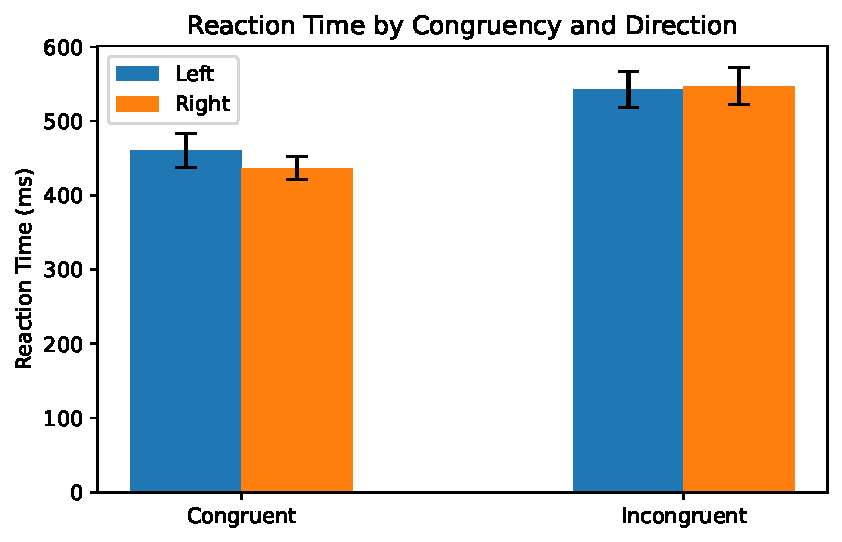
\includegraphics[keepaspectratio]{390JournalManuscript_files/figure-pdf/fig-rt-output-1.pdf}}

}

\caption{\label{fig-rt}Mean reaction time (ms) by congruency and
direction. Error bars represent ±1 SEM.}

\end{figure}%

\subsection{Accuracy}\label{accuracy}

Accuracy was higher for congruent trials (M = .97) than for incongruent
trials (M = .81) across both directions. A one-way repeated measures
ANOVA revealed a significant main effect of congruency on accuracy (F(1,
15) = 10.70, p = .005), with higher accuracy on congruent trials. A 2 x
2 repeated measures ANOVA revealed a significant main effect of
congruency on accuracy (F(1, 14) = 8.60, p = .011). There was no
significant main effect of direction (F(1, 14) = 0.52, p = .484) and no
significant interaction between congruency and direction (F(1, 14) =
0.19, p = .673). The results for the reaction time of congruent trials
compared to the incongruent trials are depicted in Figure~\ref{fig-acc}.

\begin{figure}[H]

\centering{

\pandocbounded{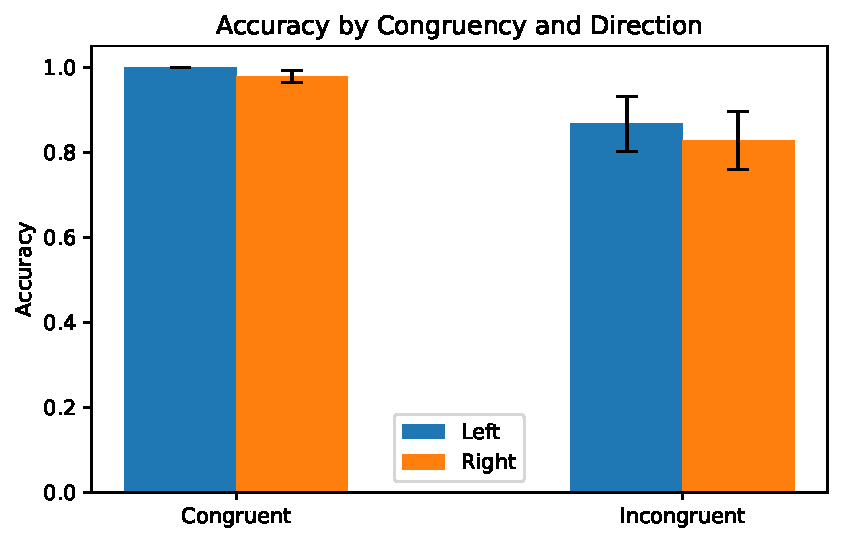
\includegraphics[keepaspectratio]{390JournalManuscript_files/figure-pdf/fig-acc-output-1.pdf}}

}

\caption{\label{fig-acc}Mean accuracy by congruency and direction. Error
bars represent ±1 SEM.}

\end{figure}%

\section{Discussion}\label{discussion}

Effect of Congruency on Performance The present study examined the
effect of stimulus congruency on response time and accuracy using a
within-subjects flanker task design. Consistent with expectations,
participants responded significantly slower and less accurately on
incongruent trials compared to congruent trials. Reaction times
increased from 477.41 ms in congruent trials to 571.28 ms in incongruent
trials, and this difference was statistically significant, F(1, 15) =
56.70, p \textless{} .001. Importantly, the F value (F = 56.70)
indicates a strong effect of congruency on response time, suggesting
that a substantial proportion of variance in reaction time is explained
by whether trials were congruent or incongruent. This reinforces that
the manipulation of congruency was highly effective in producing
interference.

\subsection{Interpretation Within Flanker and Cognitive Control
Research}\label{interpretation-within-flanker-and-cognitive-control-research}

These findings replicate the classic flanker effect first reported by
\citet{eriksen1974}, who showed that incongruent trials produce slower
responses due to response competition. In the current study, incongruent
flankers likely activated competing motor responses, requiring
participants to suppress irrelevant information and selectively attend
to the target. This supports the idea that attentional selection is not
fully efficient and that irrelevant stimuli are processed automatically,
interfering with performance \citep{eriksen1974}.

Beyond replicating the original findings, the present results are also
consistent with contemporary models of cognitive control. According to
the conflict monitoring theory, the cognitive system continuously
detects conflict between competing responses and recruits control
processing to resolve it (Bovinick et al., 2001). Incongruent trials
generate higher levels of conflict because flankers activate an opposing
response, leading to increased processing time. Conflict is associated
with activity in the anterior cingulate cortex (ACC), which plays a role
in monitoring conflict and signaling the need for increased control
\citep{botvinick2001}. The slower reaction times observed in this study
are therefore consistent with increased cognitive effort required to
resolve this conflict.

The accuracy results further strengthen this interpretation. While
participants performed well in congruent trials (M = 0.97), the accuracy
dropped substantially in incongruent trials (M= 0.81), and this
difference is statistically significant, F(1, 15) = 10.70, p = .005,
confirming that incongruent trials not only slow responses but also
significantly increase error rates. Although the effect size for
accuracy is smaller than for reaction time, it still indicates a
reliable impact on interference on performance. This dual cost, with
both speed and accuracy, has been widely reported and is considered a
hallmark of interference paradigms \citep{ridderinkhof2004}. This
reduction in accuracy suggests that, in some cases, participants failed
to fully inhibit response activated by the flankers, leading to
incorrect responses.

Importantly, the magnitude of the effect observed in this study is
comparable to previous experimental findings. For instance,
\citet{fan2002} demonstrated that incongruent trials consistently
produce slower responses in attention network paradigms, which reflected
the efficiency of executive control mechanisms. Similarly,
\citet{gratton1992} showed that interference effects in flanker tasks
are not static but can vary depending on previous trial history, a
phenomenon known as the Gratton effect. Although sequential effects were
not directly analyzed in the present study, the strong interference
observed suggests that similar adaptive control processes may be
occurring.

\subsection{Two-way Analysis: Role of
Direction}\label{two-way-analysis-role-of-direction}

The inclusion of second analysis (two-way repeated measures ANOVA)
further extends the interpretation of these findings. By incorporating
direction (left vs.~right) as a second independent variable, the design
allows for the examination of spatial influences on attention. This
approach is similar to combined flanker-Simon paradigms, where both
stimulus identity and spatial location contribute to interference
\citep{stoffels1988}. Spatial and identity-based conflicts can interact,
suggesting that multiple cognitive systems contribute to response
selection \citep{hommel1993}. Although the primary effect in the present
study was driven by congruency, future analyses could explore whether
direction interacts with congruency to produce additional interference
effects.

The two-way ANOVA results showed that the main effect of congruency on
reaction time remained a significant main effect of congruency,F(1, 14)
= 8.60, p = .011, further supporting the impact of incongruency on
performance accuracy. However, neither the main effect of direction,
F(1, 14) = 0.52, p = .484, nor the interaction between congruency and
direction, F(1, 14) = 0.19, p = .673, reached significance. These
findings indicate that accuracy differences are driven primarily by
congruency and not by spatial response factors.

Another important implication of the current findings relates to a
broader understanding of selective attention. The results support the
idea that attention operates as a limited-capacity system that must
actively filter out irrelevant information. When distractors are highly
similar or strongly associated with the response, they are more
difficult to ignore, leading to increased interference. This aligns with
evidence from electrophysiological studies showing that incongruent
trials elicit larger event-related potentials associated with conflict
processing \citep{clayson2011}. These neural findings complement
behavioural results by demonstrating that conflict processing occurs
rapidly and automatically.

\subsection{Limitations and Future
Implementations}\label{limitations-and-future-implementations}

The present study has several limitations that should be considered when
interpreting the findings. First, the small sample size (N = 16) reduces
statistical power and limits the generalizability of the results. In
addition, the use of a restricted sample of University of Waterloo
undergraduate students limits variability in demographic characteristics
such as age and education level, making the findings less representative
of the general population.

A further limitation relates to the task design. For example, each
participant completed only 20 experimental trials, which may reduce the
reliability of both reaction time and accuracy measures. With such a
small number of trials, individual variability and random fluctuations
in performance are more likely to influence overall results.
Additionally, although trials were randomly generated, this meant that
they were not fully balanced across conditions. This may have resulted
in unequal representation of congruent and incongruent trials, which
would introduce variability and reduce the precision of comparisons
between conditions.

Future research should address these limitations by increasing sample
size and recruiting more diverse participants to improve
generalizability. Moreover, increasing the number of trials and ensuring
a fully balanced design would help to enhance the reliability and
validity of the findings. Future studies could also extend this work by
examining individual differences in cognitive control across populations
to provide deeper insight into how interference effects may vary across
contexts.

Lastly, across both one-way and two-way analyses in the present study,
congruency consistently emerged as the only significant factor
influencing performance, while direction and interaction effects were
non-significant. This pattern helps to reinforce the interpretation that
cognitive interference in the flanker task is primarily driven by
response conflict rather than spatial processing.

\section{Conclusion}\label{conclusion}

Consistent with theories of selective attention and cognitive control,
the results of the present study provide clear support for the flanker
interference effect \citep{stoffels1988}. Specifically, participants
showed both slower response times and lower accuracy on incongruent
trials, indicating that flanker stimuli were automatically processed
even when they were task-irrelevant. This suggests that participants
were unable to fully suppress distracting information, highlighting the
limits of cognitive control under conditions of response conflict.

Also important to note is that the main effect of direction (left
vs.~right) was not significant, nor was the interaction between
direction and congruency, indicating that distractor congruency was the
primary driver of performance differences. This helps to strengthen the
interpretation that the observed flanker effects are due to interference
from competing stimuli rather than simple response biases.

Limitations: The small sample size (N = 16) reduces statistical power
and limits the generalizability of the findings. Additionally, the use
of a restricted sample of University of Waterloo students limits
variability in age and educational background, making the results less
representative of the broader population. The study also included only
20 trials per participant, which may reduce the reliability and
stability of both reaction time and accuracy measures. + randomized
sequences

Future Directions: Future research should address these limitations by
increasing sample size, diversifying participant demographics, and
including a greater number of trials to improve measurement reliability.
In addition, exploring individual differences in cognitive control
across populations could provide deeper insight into how interference
effects vary across contexts.

Overall, despite its limitations, this study successfully replicates a
well-established cognitive effect and demonstrates the robustness of the
flanker paradigm as a tool for studying attention and response conflict.

\section*{References}\label{references}
\addcontentsline{toc}{section}{References}

\renewcommand{\bibsection}{}
\bibliography{bibliography.bib}





\end{document}
